\chapter{Extra Information}
\section{Evaluated Knowledge Graphs}
\lstset
{
    breaklines=true,
    breakatwhitespace=false,
    basicstyle=\linespread{1}\ttfamily,
}
\begin{lstlisting}[caption={Part14\_000Brouwershaven}]
@prefix fx:   <http://sparql.xyz/facade-x/ns/> .
@prefix oont: <http://w3id.org/polifonia/ontology/organs/> .
@prefix rdf:  <http://www.w3.org/1999/02/22-rdf-syntax-ns#> .
@prefix rdfs: <http://www.w3.org/2000/01/rdf-schema#> .
@prefix wd:   <https://www.wikidata.org/wiki/> .
@prefix xyz:  <http://sparql.xyz/facade-x/data/> .

"Werkindeling\nhoofdwerk, nevenwerk, pedaal\n\nDispositie\n\nTABLE:3\n\n\nWerktuiglijke registers\nkoppelingen HW-NW, Ped-HW, Ped-NW\ntremulant\n\nSamenstelling vulstem\n\nTABLE:5\n\n\nToonhoogte\na1 = 440 Hz\nTemperatuur\nevenredig zwevend\n\nManuaalomvang\nC-f3\nPedaalomvang\nC-d1\n\nWindvoorziening\ntwee regulateurs\nWinddruk\n74 mm\n\nPlaats klaviatuur\nachterzijde"
        oont:keyboardRange      "C-f3" ;
        oont:pedalRange         "C-d1" ;
        oont:pitch              "a1 = 440 Hz" ;
        oont:systemPlayingAids  "koppelingen HW-NW, Ped-HW, Ped-NW\ntremulant" ;
        oont:temperature        "evenredig zwevend" ;
        oont:windPressure       "74 mm" ;
        oont:windSystem         "twee regulateurs" .

wd:Q12460259  oont:locationImage  <https://staticbrainz.org/irombook/reed_organ/reed_organ.png> .

"Hoofdwerk (I)"  oont:extraInformation  <https://organhistoricalsociety.org/OrganHistory/works/works05.htm> .

"Gereformeerde Kerk Vrijgemaakt"
        oont:extraInformation  <https://nl.wikipedia.org/wiki/Gereformeerde_Kerk_Vrijgemaakt> .

"74 mm"  oont:extraInformation  <https://organhistoricalsociety.org/OrganHistory/works/works06.htm> .

"twee regulateurs"  oont:extraInformation
                <https://organhistoricalsociety.org/OrganHistory/works/works06.htm> .

"a1 = 440 Hz"  oont:extraInformation  <https://organhistoricalsociety.org/OrganHistory/works/works04.htm> .

"disposition"  xyz:divisionName       "Hoofdwerk (I)" ;
        oont:AdditionalSpecification  "8'" ;
        oont:partition                "" .

"Brouwershaven"  oont:extraInformation  <https://nl.wikipedia.org/wiki/Brouwershaven> .

"Part14_000Brouwershaven"
        rdf:type               oont:Organ , wd:Q173453 ;
        rdfs:subClassOf        wd:Q12460259 , wd:Q1327327 , wd:Q281460 , wd:Q752638 ;
        xyz:change             "orgel buiten gebruik gesteld" ;
        xyz:disposition        "disposition" ;
        xyz:technicals         "Werkindeling\nhoofdwerk, nevenwerk, pedaal\n\nDispositie\n\nTABLE:3\n\n\nWerktuiglijke registers\nkoppelingen HW-NW, Ped-HW, Ped-NW\ntremulant\n\nSamenstelling vulstem\n\nTABLE:5\n\n\nToonhoogte\na1 = 440 Hz\nTemperatuur\nevenredig zwevend\n\nManuaalomvang\nC-f3\nPedaalomvang\nC-d1\n\nWindvoorziening\ntwee regulateurs\nWinddruk\n74 mm\n\nPlaats klaviatuur\nachterzijde" ;
        oont:builder           "A.S.J. Dekker" ;
        oont:consolelocation   "" ;
        oont:creator           "Een vijfdelig front met spitse zijtorens, een halfronde middentoren en relatief brede tussenvelden op verhoogde pijpstok. Aan bovenzijde lopen de pijpvelden schuin op naar de middentoren, waarbij de gebogen lijn aan het einde wordt afgesloten met een knop. Het pijpwerk is aan boven- en onderzijde geblindeerd, met vormen die doen denken aan de contour van een liggende C-voluut. Bij de blinderingen van de torens zijn fraaie accenten aangebracht. Onder lopen de blinderingen uit in een smalle punt in midden, boven in een hangende lelie. De torens zijn bekroond met koepels met daarop een bol, waarbij de koepels worden geflankeerd door kleine obelisken op sokkels. De vleugelstukken zijn samengesteld uit een S-voluut met krullen en onder andere twee hoorns. Bij het oorspronkelijke ontwerp maakte de onderkas zeer waarschijnlijk deel uit van een doorlopend balkon in dezelfde vormentaal, zoals te zien is bij het vrijwel identieke Dekkerorgel te Simonshaven.)" ;
        oont:dateOfBirth       "1910" ;
        oont:extraInformation  wd:Q1444 ;
        oont:history           "Bouwers\n1. A.S.J. Dekker\n2. H.J. Vierdag\n\nJaren van oplevering\n1. 1910\n2. 1978\n\nDispositie 1910\n\nTABLE:1\n\n\noctaafkoppel\naangehangen pedaal\n\n1970\n.orgel buiten gebruik gesteld\n\nH.J. Vierdag 1978\n.nieuw orgel in oude kas met gebruikmaking van enig oud pijpwerk" ;
        oont:monument          "Gereformeerde Kerk Vrijgemaakt" ;
        oont:monumentNumber    "" ;
        oont:moreInformation   "Victor Timmer & Ton van Eck, ‘Twee werklijsten van orgelmakers uit de eerste helft van de 20ste eeuw. De firma A.S.J. Dekker en de door haar overgenomen ‘Orgelfabriek P. van Dam’. Het Orgel, 101/3 (2005), 27." ;
        oont:name              "Brouwershaven, Gereformeerde Kerk Vrijgemaakt" ;
        oont:organNumber       "" ;
        oont:particularities   "De firma A.S.J. Dekker leverde in maart 1910 een nieuw pneumatisch orgel op in de (toen nog) Gereformeerde Kerk van Brouwershaven. Van dit instrument resteert naast de orgelkas nog pijpwerk in de registers Prestant 8' en Octaaf 4' (HW), alsmede Holpijp 8' en Fluit 4' (NW).\nVan de Prestant 8' staan C-b in het front en h-f3 op de lade; alle binnenpijpen met expressions. De Octaaf 4' dateert van C-f2 uit 1910 (met expressions) de overige pijpen zijn in 1978 vernieuwd. De Fluit 4' (NW) is van C-f2 van metaal (gedekt, 1910), het vervolg is open, conisch (1978)." ;
        oont:state             "Brouwershaven" .

wd:Q1444  wd:Property:P1343  wd:Q106727050 , wd:Q302556 ;
        wd:Property:P1535  wd:Q765778 ;
        wd:Property:P1709  <https://dbpedia.org/ontology/Organ> ;
        wd:Property:P1889  wd:Q281460 ;
        wd:Property:P2579  wd:Q11163731 ;
        wd:Property:P279   wd:Q19603939 , wd:Q52954 ;
        wd:Property:P3095  wd:Q1495811 ;
        wd:Property:P366   wd:Q60733114 , wd:Q9730 ;
        wd:Property:P527   wd:Q2927648 , wd:Q1446290 , wd:Q901207 , wd:Q25112583 , wd:Q1510738 , wd:Q392573 , wd:Q1758965 .

""      oont:extraInformation  <https://nl.wikipedia.org/wiki/> .

"orgel buiten gebruik gesteld"
        oont:AdditionalSpecification  "1970" ;
        oont:Builder                  "" ;
        oont:date                     "1970" .
\end{lstlisting} 

\lstset
{
    breaklines=true,
    breakatwhitespace=false,
    basicstyle=\linespread{1}\ttfamily,
}
\begin{lstlisting}[caption={Part14\_000Niezijl}]
@prefix fx:   <http://sparql.xyz/facade-x/ns/> .
@prefix oont: <http://w3id.org/polifonia/ontology/organs/> .
@prefix rdf:  <http://www.w3.org/1999/02/22-rdf-syntax-ns#> .
@prefix rdfs: <http://www.w3.org/2000/01/rdf-schema#> .
@prefix wd:   <https://www.wikidata.org/wiki/> .
@prefix xyz:  <http://sparql.xyz/facade-x/data/> .

wd:Q12460259  oont:locationImage  <https://staticbrainz.org/irombook/reed_organ/reed_organ.png> .

"a1 = 435 Hz"  oont:extraInformation  <https://organhistoricalsociety.org/OrganHistory/works/works04.htm> .

"Gereformeerde Kerk Vrijgemaakt"
        oont:extraInformation  <https://nl.wikipedia.org/wiki/Gereformeerde_Kerk_Vrijgemaakt> .

"Werkindeling\nmanuaal, aangehangen pedaal\n\nDispositie\n\nTABLE:1\n\n\nWerktuiglijke registers\nknop voor inschakelen C-H Bourdon 16'\ntremulant\n\n\nSamenstelling vulstem\nCornet   c1   8 - 4 - 2 2/3 - 2 - 1 3/5\n\nToonhoogte\na1 = 435 Hz\nTemperatuur\nevenredig zwevend\n\nManuaalomvang\nC-f3\nPedaalomvang\nC-c1\n\nWindvoorziening\nmagazijnbalg met inspringende vouw, twee schepbalgen en handpomp (1907)\nWinddruk\n65 mm\n\nPlaats klaviatuur\nrechterzijde"
        oont:keyboardRange      "C-f3" ;
        oont:pedalRange         "C-c1" ;
        oont:pitch              "a1 = 435 Hz" ;
        oont:systemPlayingAids  "knop voor inschakelen C-H Bourdon 16'\ntremulant" ;
        oont:temperature        "evenredig zwevend" ;
        oont:windPressure       "65 mm" ;
        oont:windSystem         "magazijnbalg met inspringende vouw, twee schepbalgen en handpomp (1907)" .

"Niezijl"  oont:extraInformation  <https://nl.wikipedia.org/wiki/Niezijl> .

"Part14_000Niezijl"  rdf:type  wd:Q173453 , oont:Organ ;
        rdfs:subClassOf        wd:Q12460259 , wd:Q1327327 , wd:Q281460 , wd:Q752638 ;
        xyz:change             "herstel" ;
        xyz:disposition        "disposition" ;
        xyz:technicals         "Werkindeling\nmanuaal, aangehangen pedaal\n\nDispositie\n\nTABLE:1\n\n\nWerktuiglijke registers\nknop voor inschakelen C-H Bourdon 16'\ntremulant\n\n\nSamenstelling vulstem\nCornet   c1   8 - 4 - 2 2/3 - 2 - 1 3/5\n\nToonhoogte\na1 = 435 Hz\nTemperatuur\nevenredig zwevend\n\nManuaalomvang\nC-f3\nPedaalomvang\nC-c1\n\nWindvoorziening\nmagazijnbalg met inspringende vouw, twee schepbalgen en handpomp (1907)\nWinddruk\n65 mm\n\nPlaats klaviatuur\nrechterzijde" ;
        oont:builder           "M. Eertman" ;
        oont:consolelocation   "" ;
        oont:creator           "Dit front is nagenoeg identiek aan dat te Ten Boer (Gereformeerde Kerk 1907). Er zijn slechts enkele verschillen in de decoratie. Zo ontbreken hier de ornamenten onder de torens en de opstaande bladvoluten tegen de middelste torenkap. De torenbekroningen zijn anders en bestaan hier uit een lier en twee geoorde vazen. De vleugelstukken zijn opgebouwd uit een samenstel van S- en C-vormige bladvoluten, waartussen deze keer geen trofee van muziekinstrumenten is opgenomen." ;
        oont:dateOfBirth       "1907" ;
        oont:extraInformation  wd:Q1444 ;
        oont:history           "Bouwer\nM. Eertman\n\nJaar van oplevering\n1907\n\nHoltman & Leemshuis 1947\n.herstel\n\nHoltman & Leemhuis 1959\n.herstel\n\nJ.J. Harkema 1968\n.orgel gewijzigd\n.nieuw handklavier; registerknoppen verplaatst\n.Salicionaal 8' ◂ Quint 3'; bas Bourdon 16' op pneumatische lade geplaatst\n\n1972\n.orgel ernstig beschadigd door lekkage en vervolgens buiten gebruik gesteld\n\n1977\n.orgelkas opnieuw geschilderd\n\nGebr. Reil 1983\n.restauratie\n.tremulant toegevoegd\n.mechanieken gerestaureerd; nieuwe registerknoppen aangebracht\n.windlade gerestaureerd; sleep Trompet 8' gedeeld, Bourdon 16' van twee standen voorzien\n.bas Bourdon 16' weer op lade Man geplaatst; Quint 3' vervangen\n\nF.R. Feenstra 1996\n.windvoorziening gerestaureerd" ;
        oont:monument          "Gereformeerde Kerk Vrijgemaakt" ;
        oont:monumentNumber    "" ;
        oont:moreInformation   "Het Groninger Orgelbezit van Adorp tot Zijldijk. 2 Westerkwartier, Groningen (1995), 126-127.\nDe Mixtuur, 42 (1983), 488." ;
        oont:name              "Niezijl, Gereformeerde Kerk Vrijgemaakt" ;
        oont:organNumber       "1065" ;
        oont:particularities   "Deling B/D tussen h en c1.\nDe orgelkas is sinds 1977 geschilderd in een houtimitatie, voorheen was de kas wit. Het dak van de kas is vlak en heeft in het midden een afdekking met gasdoek, waar normaal de behuizing achter de kap van de middentoren zou zitten. De bovenste tussenvelden bevatten stomme zinken pijpen, op lengte afgesneden.\nDe magazijnbalg ligt links naast het orgel. De schepbalgen en handpomp zijn in 1996 verwijderd. De tremulant is pneumatisch.\nDe registerknoppen bevinden zich vlak onder de lessenaarbak; de trekstokken zijn rond. Rechts boven de lessenaarbak zijn aan de binnenzijde van de kas vier ronde gedichte gaten zichtbaar met dezelfde maat als die van de gewone registertrekkers; zijn dit sporen van een vroegere vrije combinatie of van een nooit geplaatst bovenwerk?\nBoven de knop van de Bourdon bevindt zich een houten palletje waarmee het mogelijk is dit register in- of uit te schakelen.\nHet pijpwerk staat op een laagliggende C- en Cislade. In het midden staan - van achteren gezien - [als we de deling in twee laden wegdenken] C-A in hele tonen naar weerszijden aflopend; aan de uiteinden van de lade B-h en de discant daar tussenin. Beide laden hebben twee eiken opliggende voorslagen, elk vastgezet met twee voorslagijzers. Tussen laden en vloer ligt een eiken walsraam met veelhoekige grenen walsen en metalen walsarmpjes.\nHet meeste metalen pijpwerk heeft geperste labia en expressions. De Prestant 8' staat van C-g1 in het front (torens en onderste tussenvelden, zink), het vervolg staat op de lade, metaal. De Bourdon 16' is geheel van hout (geverfd), deels afgevoerd. C-B van de Roerfluit 8' zijn van hout met doorboorde stoppen, h-f3 metaal, gedekt met inwendige roeren. C-H van de Gamba 8' zijn van zink, het vervolg is van orgelmetaal. De Octaaf 4' bestaat uit ouder pijpwerk (spitsboog gedrukt bovenlabium); C-f1 met expressions, het vervolg is op lengte afgesneden. De Quint 3' is geheel van metaal. De Flûte Travers 4' is geheel metaal, open. Het acht-voets koor van de Cornet is gedekt, met ronde houten stoppen en handvatten; alleen de kleinste pijpjes van het 1 3/5-voets koor zijn op lengte afgesneden. De Gemshoorn 2' is van metaal, licht conisch; alleen de kleinste 12 zijn op lengte afgesneden. De Trompet 8' heeft zinken stevels en bekers voor C-H (met intonatie uitsnijdingen); het vervolg is van metaal. C-d1 hebben versterkte onderkant bekers. Benaming bas op de betreffende registerknop als basc." ;
        oont:state             "Niezijl" .

"Manuaal"  oont:extraInformation  <https://organhistoricalsociety.org/OrganHistory/works/works05.htm> .

"65 mm"  oont:extraInformation  <https://organhistoricalsociety.org/OrganHistory/works/works06.htm> .

"herstel"  oont:AdditionalSpecification
                "Holtman & Leemshuis 1947" ;
        oont:Builder                  "Holtman & Leemshuis" ;
        oont:date                     "1947" .

"disposition"  xyz:divisionName       "Manuaal" ;
        oont:AdditionalSpecification  "16" ;
        oont:partition                "" .

"magazijnbalg met inspringende vouw, twee schepbalgen en handpomp (1907)"
        oont:extraInformation  <https://organhistoricalsociety.org/OrganHistory/works/works06.htm> .

"Holtman & Leemshuis"
        oont:extraInformation  <https://nl.wikipedia.org/wiki/Holtman_&_Leemshuis> .

wd:Q1444  wd:Property:P1343  wd:Q106727050 , wd:Q302556 ;
        wd:Property:P1535  wd:Q765778 ;
        wd:Property:P1709  <https://dbpedia.org/ontology/Organ> ;
        wd:Property:P1889  wd:Q281460 ;
        wd:Property:P2579  wd:Q11163731 ;
        wd:Property:P279   wd:Q19603939 , wd:Q52954 ;
        wd:Property:P3095  wd:Q1495811 ;
        wd:Property:P366   wd:Q60733114 , wd:Q9730 ;
        wd:Property:P527   wd:Q2927648 , wd:Q1446290 , wd:Q901207 , wd:Q25112583 , wd:Q1510738 , wd:Q392573 , wd:Q1758965 .
\end{lstlisting}

\lstset
{
    breaklines=true,
    breakatwhitespace=false,
    basicstyle=\linespread{1}\ttfamily,
}
\begin{lstlisting}[caption={Part14\_000Folsgare}]
@prefix fx:   <http://sparql.xyz/facade-x/ns/> .
@prefix oont: <http://w3id.org/polifonia/ontology/organs/> .
@prefix rdf:  <http://www.w3.org/1999/02/22-rdf-syntax-ns#> .
@prefix rdfs: <http://www.w3.org/2000/01/rdf-schema#> .
@prefix wd:   <https://www.wikidata.org/wiki/> .
@prefix xyz:  <http://sparql.xyz/facade-x/data/> .

"Part14_000Folsgare"  rdf:type  oont:Organ , wd:Q173453 ;
        rdfs:subClassOf        wd:Q752638 , wd:Q1327327 , wd:Q281460 , wd:Q12460259 ;
        xyz:change             "orgel overgeplaatst naar nieuw kerkgebouw" ;
        xyz:disposition        "disposition" ;
        xyz:technicals         "Werkindeling\nmanuaal, aangehangen pedaal\n\nDispositie\n\nTABLE:1\n\n\nWerktuiglijk register\ntremulant\n\nSamenstelling vulstem\n\nTABLE:3\n\n\nToonhoogte\na1 = 432 Hz\nTemperatuur\nevenredig zwevend\n\nManuaalomvang\nC-f3\nPedaalomvang\nC-d1\n\nWindvoorziening\nmagazijnbalg\nWinddruk\n62 mm\n\nPlaats klaviatuur\nlinkerzijde" ;
        oont:builder           "Bakker & Timmenga" ;
        oont:consolelocation   "Marrum, Gereformeerde Kerk" ;
        oont:creator           "Een acht-voets variant van het bekende Bakker & Timmenga-front dat in 1894 voor het eerst in het oeuvre van deze orgelmakers verscheen. De grotere breedtemaat is ontstaan door de maten van de grotere frontpijpen en de plaatsing van negen pijpen in de velden. Hierdoor kon een volledige Bourdon 16' worden gedisponeerd. De velden zijn vlak uitgevoerd, gescheiden door een brede lijst met licht gebogen onderkant, het labiumverloop van de veldpijpen is parallel.\nDe ornamenten volgen het voor dit fronttype vaste patroon: plantaardige motieven in de blinderingen, acanthusmotieven in de culs-de-lampe, opengewerkte opzetstukken op de torenkappen, waarbij de middentoren tevens een lier draagt.\nDe vleugelstukken vertonen de bekende compositie van S- en C-voluutbanden, omrankt met wijnrank en vogeltje. Opmerkelijk is het kleurverschil tussen blinderingen en culs-de-lampe enerzijds en opzetstukken met vleugels anderzijds." ;
        oont:dateOfBirth       "1908" ;
        oont:extraInformation  wd:Q1444 ;
        oont:history           "Bouwer\nBakker & Timmenga\n\nJaar van oplevering\n1908\n\nOorspronkelijke locatie\nMarrum, Gereformeerde Kerk\n\nBakker & Timmenga 1924\n.orgel overgeplaatst naar nieuw kerkgebouw\n.Holpijp van nieuwe hoeden voorzien\n\nBakker & Timmenga 1926\n.registerknoppen verplaatst\n.+ Trompet 8' (inclusief sleep, stok en registermechaniek) op daarvoor gereserveerde plaats\n\nBakker & Timmenga 1934\n.tremulant toegevoegd\n\nBakker & Timmenga 1935\n.stoppen houten pijpen van viltpakkingen voorzien\n\nOrgelmakerij Ernst Leeflang 1964\n.orgel overgeplaatst naar Folsgare, Hervormde Kerk\n.pedaalklavier vernieuwd\n.nieuwe, kleinere magazijnbalg aangebracht\n.- Cornet D 3 st., + Mixtuur 2-3 st." ;
        oont:monument          "Hervormde Kerk" ;
        oont:monumentNumber    "39762" ;
        oont:moreInformation   "Jan Jongepier, Vijf eeuwen Friese orgelbouw. Leeuwarden, 2004, 186.\n\nNiet gepubliceerde bron\nArchief Orgelmakerij Bakker & Timmenga, Leeuwarden, HCL." ;
        oont:name              "Folsgare (Folsgeare), Hervormde Kerk" ;
        oont:organNumber       "264" ;
        oont:particularities   "Deling B/D Bourdon 16' tussen H en c.\nDe frontpijpen zijn van metaal met een hoog tingehalte. Sprekend (Prestant 8' vanaf C) zijn de drie torens en in de onderste tussenvelden aan weerskanten de eerste vier, (C-kant) respectievelijk vijf (Cis-kant) pijpen, gerekend vanaf de middentoren.\nHet handklavier is een eiken staartklavier met celluloidbeleg op de ondertoetsen. De verplaatste registerknoppen dateren (behalve die van de tremulant) nog uit 1908. Aan de binnenzijde van de kas zijn de oorspronkelijke registergaten boven de lessenaar nog zichtbaar. Het pedaalklavier heeft vanuit het midden naar buiten toe boventoetsen van oplopende lengte. Het oorspronkelijk pedaalklavier had een omvang van C-g. De in 1964 geleverde registerknop voor de Mixtuur is een knop van Witte met als opschrift Mixtuur 2 vt, en is naar alle waarschijnlijkheid afkomstig van het Witte orgel in de Gereformeerde Kerk te Anjum (oorspronkelijk Utrecht, Remonstrantse kerk, 1866 en kort voor 1964 door Leeflang gemoderniseerd en gewijzigd).\nDe balg ligt in de onderkas, de windmachine is op die plaats naast de balg opgesteld. Oorspronkelijk bezat de magazijnbalg met schepbalgen een handpomp die in klampen tegen de achterwand was aangebracht. De openingen voor de hefbomen en het windzicht zijn dichtgezet. De schuif voor het ventiel, op een voorslag gemonteerd, is er nog, maar dient nu de pneumatische bediening van de tremulant. Het bestek van l908 vermeldt een winddruk van 75 mm.\nDe windlade is van eiken, maar stokken en roosters zijn van mahonie. De ventielkast heeft drie opliggende, vastgeschroefde voorslagen. De cancelvolgorde is: fis d B Fis c e gis / e3 (hele tonen) b / Fis E D C Cis Dis F / a (hele tonen) f3 / g dis H Gis A cis f. (f aan klavierzijde).\nHouten pijpen van Amerikaans grenen zijn toegepast voor de Bourdon 16' (C-h, waarvan C-G tegen de rechter zijkant opgesteld en voorzien van voorbaarden) en de Holpijp 8' (C-H). De Viola di Gamba 8' is van C-H gecombineerd met de Holpijp en verder van tin. De Fluit 4' is gedekt, het hoogste octaaf is echter open, conisch.\nDe Trompet 8' heeft zinken stevels en zinken bekers. Alle inscripties zijn met slagletters uitgevoerd, de registernaam luidt Trompete. De koppen zijn van lood. Alle bekers zijn van slitsen voorzien.\nAl het metalen binnenpijpwerk is toegeleverd materiaal. Het merendeel hiervan heeft geperste labia. Het pijpwerk van de Holpijp heeft spits geritste labia en pijpwanden die door hun speciale structuur als spotted worden aangeduid. Expressions zijn toegepast bij alle pijpen van Prestant en Viola di Gamba, bij de Octaaf 4' (C-f2) en bij de Octaaf 2' (C-cis1)." ;
        oont:state             "Folsgare (Folsgeare)" .

wd:Q12460259  oont:locationImage  <https://staticbrainz.org/irombook/reed_organ/reed_organ.png> .

"Folsgare (Folsgeare)"
        oont:extraInformation  <https://nl.wikipedia.org/wiki/Folsgare_(Folsgeare)> .

"a1 = 432 Hz"  oont:extraInformation  <https://organhistoricalsociety.org/OrganHistory/works/works04.htm> .

"Manuaal"  oont:extraInformation  <https://organhistoricalsociety.org/OrganHistory/works/works05.htm> .

"orgel overgeplaatst naar nieuw kerkgebouw"
        oont:AdditionalSpecification  "Bakker & Timmenga 1924" ;
        oont:Builder                  "Bakker & Timmenga" ;
        oont:date                     "1924" .

"Werkindeling\nmanuaal, aangehangen pedaal\n\nDispositie\n\nTABLE:1\n\n\nWerktuiglijk register\ntremulant\n\nSamenstelling vulstem\n\nTABLE:3\n\n\nToonhoogte\na1 = 432 Hz\nTemperatuur\nevenredig zwevend\n\nManuaalomvang\nC-f3\nPedaalomvang\nC-d1\n\nWindvoorziening\nmagazijnbalg\nWinddruk\n62 mm\n\nPlaats klaviatuur\nlinkerzijde"
        oont:keyboardRange      "C-f3" ;
        oont:pedalRange         "C-d1" ;
        oont:pitch              "a1 = 432 Hz" ;
        oont:systemPlayingAids  "tremulant" ;
        oont:temperature        "evenredig zwevend" ;
        oont:windPressure       "62 mm" ;
        oont:windSystem         "magazijnbalg" .

"disposition"  xyz:divisionName       "Manuaal" ;
        oont:AdditionalSpecification  "8'" ;
        oont:partition                "B/D" .

"Hervormde Kerk"  oont:extraInformation
                <https://nl.wikipedia.org/wiki/Hervormde_Kerk> .

"magazijnbalg"  oont:extraInformation  <https://organhistoricalsociety.org/OrganHistory/works/works06.htm> .

"62 mm"  oont:extraInformation  <https://organhistoricalsociety.org/OrganHistory/works/works06.htm> .

wd:Q1444  wd:Property:P1343  wd:Q106727050 , wd:Q302556 ;
        wd:Property:P1535  wd:Q765778 ;
        wd:Property:P1709  <https://dbpedia.org/ontology/Organ> ;
        wd:Property:P1889  wd:Q281460 ;
        wd:Property:P2579  wd:Q11163731 ;
        wd:Property:P279   wd:Q19603939 , wd:Q52954 ;
        wd:Property:P3095  wd:Q1495811 ;
        wd:Property:P366   wd:Q60733114 , wd:Q9730 ;
        wd:Property:P527   wd:Q2927648 , wd:Q1446290 , wd:Q901207 , wd:Q25112583 , wd:Q1510738 , wd:Q392573 , wd:Q1758965 .

"Bakker & Timmenga"  oont:extraInformation
                <https://nl.wikipedia.org/wiki/Bakker_&_Timmenga> .
\end{lstlisting}

\lstset
{
    breaklines=true,
    breakatwhitespace=false,
    basicstyle=\linespread{1}\ttfamily,
}
\begin{lstlisting}[caption={Part14\_000GravenhageNoorderkerk}]
@prefix fx:   <http://sparql.xyz/facade-x/ns/> .
@prefix oont: <http://w3id.org/polifonia/ontology/organs/> .
@prefix rdf:  <http://www.w3.org/1999/02/22-rdf-syntax-ns#> .
@prefix rdfs: <http://www.w3.org/2000/01/rdf-schema#> .
@prefix wd:   <https://www.wikidata.org/wiki/> .
@prefix xyz:  <http://sparql.xyz/facade-x/data/> .

"HW en pneumatiek 110 mm, Ped 98 mm, ZwW 94 mm"
        oont:extraInformation  <https://organhistoricalsociety.org/OrganHistory/works/works06.htm> .

wd:Q12460259  oont:locationImage  <https://staticbrainz.org/irombook/reed_organ/reed_organ.png> .

"a1 = 435 Hz"  oont:extraInformation  <https://organhistoricalsociety.org/OrganHistory/works/works04.htm> .

"Werkindeling\nmanuaal I, manuaal II, pedaal\n\nDispositie\n\nTABLE:3\n\n\nWerktuiglijke registers\nkoppelingen I-II, I-II 16', I-II 4', Ped-I, Ped-II\nautomatisch pedaal (vrij instelbaar)\nvaste combinaties P MF F Tutti\nvrije combinatie.\ntremulant II\ntrede zwelkast Man II\n\nSamenstelling vulstemmen\n\nTABLE:5\n\n\nCornet HW   c1   4 - 2 2/3 - 2 - 1 3/5\n\n\nTABLE:7\n\n\n\nTABLE:9\n\n\nToonhoogte\na1 = 435 Hz\nTemperatuur\nevenredig zwevend\n\nManuaalomvang\nC-f3\nPedaalomvang\nC-d1\n\nWindvoorziening\ndrie magazijnbalgen\nWinddruk\nHW en pneumatiek 110 mm, Ped 98 mm, ZwW 94 mm\n\nPlaats klaviatuur\nvoorzijde"
        oont:keyboardRange      "C-f3" ;
        oont:pedalRange         "C-d1" ;
        oont:pitch              "a1 = 435 Hz" ;
        oont:systemPlayingAids  "koppelingen I-II, I-II 16', I-II 4', Ped-I, Ped-II\nautomatisch pedaal (vrij instelbaar)\nvaste combinaties P MF F Tutti\nvrije combinatie.\ntremulant II\ntrede zwelkast Man II" ;
        oont:temperature        "evenredig zwevend" ;
        oont:windPressure       "HW en pneumatiek 110 mm, Ped 98 mm, ZwW 94 mm" ;
        oont:windSystem         "drie magazijnbalgen" .

"G. van Leeuwen"  oont:extraInformation
                <https://nl.wikipedia.org/wiki/G._van_Leeuwen> .

"Part14_000GravenhageNoorderkerk"
        rdf:type               wd:Q173453 , oont:Organ ;
        rdfs:subClassOf        wd:Q12460259 , wd:Q752638 , wd:Q1327327 , wd:Q281460 ;
        xyz:change             "orgel hersteld en gewijzigd" ;
        xyz:disposition        "disposition" ;
        xyz:technicals         "Werkindeling\nmanuaal I, manuaal II, pedaal\n\nDispositie\n\nTABLE:3\n\n\nWerktuiglijke registers\nkoppelingen I-II, I-II 16', I-II 4', Ped-I, Ped-II\nautomatisch pedaal (vrij instelbaar)\nvaste combinaties P MF F Tutti\nvrije combinatie.\ntremulant II\ntrede zwelkast Man II\n\nSamenstelling vulstemmen\n\nTABLE:5\n\n\nCornet HW   c1   4 - 2 2/3 - 2 - 1 3/5\n\n\nTABLE:7\n\n\n\nTABLE:9\n\n\nToonhoogte\na1 = 435 Hz\nTemperatuur\nevenredig zwevend\n\nManuaalomvang\nC-f3\nPedaalomvang\nC-d1\n\nWindvoorziening\ndrie magazijnbalgen\nWinddruk\nHW en pneumatiek 110 mm, Ped 98 mm, ZwW 94 mm\n\nPlaats klaviatuur\nvoorzijde" ;
        oont:builder           "J. Proper" ;
        oont:consolelocation   "" ;
        oont:creator           "Een ongewoon orgelfront in het oeuvre van Proper. Er zijn geen concrete voorbeelden in zijn eerdere werk. Mogelijk is de kas door een ander ontworpen. Er is sprake van een neobarok front met een vijfdelig hoofdwerk en een loos driedelig rugwerk in de balustrade.\nHet hoofdwerkfront bezit halfronde torens, waarvan de middelste breder en hoger is, en gedeelde tussenvelden. Merkwaardig zijn de strakke schuin oplopende lijsten tussen zijtorens en middentoren, die in tegenspraak zijn met de overige barokke vormen. Het decoratieve snijwerk aan dit orgelfront is steeds gesloten gehouden. Het blinderingssnijwerk van de middentoren bestaat aan de onderzijde uit naar buiten toe oplopend gebladerte, in het midden voorzien van een opstaand lelievormig blad. Aan de bovenzijde van dezelfde toren een gevleugelde engelenkop. De zijtorens bezitten slechts aan de bovenzijde blinderingen, die bestaan uit gebogen bladranken en een centrale afhangende bloem. De onderste tussenvelden zijn rondbogig en in de boog voorzien van draperieën. De lijsten, die de bovenste tussenvelden omvatten, zijn gevuld met snijwerk van gebladerte. In de torenkappen, tegen de uiteinden van de friezen, ingekaste rozetten. Op de zijtorens opstaande palmetten tussen neerliggende S-ranken. De palmetten worden bekroond door een toorts en twee omhoogstekende bazuinen. Op de middentoren een omstraalde lier tussen twee neerliggende bladranken. Alleen onder de zijtorens consoles van acanthusbladeren.\nHet driedelige rugwerkfront bestaat uit een halfronde middentoren, geflankeerd door twee lagere rechthoekige velden. De blinderingen aan onder- en bovenzijde van torens en velden worden gevormd door gebogen bladranken met centrale uitstulpingen. Op de zijvelden liggen twee gebogen ranken tegen de middentoren; op de middentoren een adelaar met gespreide vleugels. Het rugwerk is opgenomen in een balustrade met een gesloten borstwering van rechthoekige panelen, waarboven een open hekwerk en een brede bovenlijst." ;
        oont:dateOfBirth       "1907" ;
        oont:extraInformation  wd:Q1444 ;
        oont:history           "Bouwer\nJ. Proper\n\nJaar van oplevering\n1907\n\nDispositie 1907\n\nTABLE:1\n\n\nG. van Leeuwen 1937\n.orgel hersteld en gewijzigd\n.klaviatuur verplaatst van linkerzijde naar voorzijde hoofdkas\n.dispositiewijzigingen:\nHW Cornet D 4 st. ◂ Mixtuur-Cornet\nBW + Cromorne 8'\nPed Trompet 8' ◂ Fagot 16' met 12 nieuwe pijpen (halve bekerlengte) voor C-H\n\nValckx & Van Kouteren 1953\n.orgel gewijzigd en uitgebreid met aanvullingsladen voor HW en ZwW\n.nieuwe zwelramen ZwW\n.dispositiewijzigingen:\nHW - Roerfluit 4' (naar ZwW, - Mixtuur-Cornet, + Nachthoorn 4', + Mixtuur 3-5 st., + Cornet D 4 st.; Violon 8' ◂ Salicionaal 8'\nZwW Voix Céleste 8' ◂ Terts 1 3/5', - Flûte harmonique 4', + Roerfluit 4' (van HW), - Gemshoorn 2'; op nieuwe lade + Prestant 4', + Nasard 2 2/3', + Woudfluit 2', + Scherp 3 st., Cromorne 8' ◂ Dulciaan 8'\nPed - Violon 16', Cello 8' ◂ Koraalbas 4', + Octaafbas 8', + Ruispijp 2 st., + Basson 8' (tr uit Fagot)" ;
        oont:monument          "Gereformeerde Noorderkerk" ;
        oont:monumentNumber    "" ;
        oont:moreInformation   "Organist en Eredienst, 19/211 (1953), ..\nR. Walsma, Herziene en uitgebreide werklijst Properorgels. Leeuwarden, 2005, 5.\nR. Walsma, Jan Proper (1853-1922), orgelbouwer op het grensvlak van ambachtelijk en industrieel. Leeuwarden, 2005.\n\nNiet gepubliceerde bronnen\nArchief Pels & Van Leeuwen Orgelbouw.\nSKKN, dossier Den Haag GKN Noorderkerk, inventarisrapport 1997." ;
        oont:name              "‘s-Gravenhage, Gereformeerde Noorderkerk" ;
        oont:organNumber       "" ;
        oont:particularities   "Het orgel heeft kegelladen met pneumatische tractuur.\nDe drie magazijnbalgen hebben elk één vouw. Tenzij anders aangegeven is het pijpwerk open, cilindrisch en van orgelmetaal. Het metalen pijpwerk heeft, tenzij anders vermeld , geperste labia. Indien niet anders vermeld dateert het pijpwerk uit 1907.\nDe oorspronkelijke lade van het HW is als volgt ingedeeld:\na f cis A H dis g, f3 dis3-cis1 h, G F Dis Cis C D E Fis Gis, c1 d1-d3 e3, gis e c Bes d fis b\nDe supplementlade voor de Cornet is chromatisch ingedeeld; de supplementlade voor de Mixtuur is eveneens chromatisch ingedeeld; C-h van voor naar achter en c1-f3 in tegenbeweging.\nDe Prestant 8' staat van C-dis1 in het front; e1-a1 staan achter het front op aparte laden, de overige pijpen staan op de lade. Alle pijpen met expressions. C-h van de Bourdon 16' zijn van eiken (gedekt), het vervolg is van metaal met zijbaarden. C-F staan opgesteld in de nis links van het orgel bij enkele pedaalregisters (originele toestand). De Salicionaal 8' is geheel voorzien van expressions, C-h2 met zijbaarden; dit is de milder geïntoneerde Violon uit 1907. C-H van de Roerfluit 8' zijn van eiken (gedekt), het vervolg is van metaal met roeren en zijbaarden. De Nachthoorn 4' bevat gedeeltelijk in 1953 ingekorte pijpen van de Flûte harmonique 4' (1907, ZwW). C-d1 gedekt, dis1-g2 roergedekt met inwendige roeren, gis2-f3 open conisch, zonder steminrichting. De Trompet 8' heeft Duitse koppen lepels en tongen; c3-f3 met dubbele bekerlengte. Expressions zijn aangebracht bij de registers Prestant 8' (geheel), Salicionaal 8' (geheel), Octaaf 4' (C-f2), Quint 2 2/3' (C-h1) en Octaaf 2' (C-f1); de Mixtuur en de Cornet dateren beide uit 1953 en zijn deels voorzien van expressions. Het overige open labiaalpijpwerk is op lengte afgesneden.\nDe oorspronkelijke lade van het ZwW ligt achter die van het HW. Deze lade is chromatisch ingedeeld met de registerkast tussen H en c. Op deze lade staan achtereenvolgens de registers Roerfluit 4', Bourdon 8', Viola di Gamba 8', Echo Prestant 8' en Terts 1 3/5'. Op de chromatisch ingedeelde zijlade staan de overige stemmen die allemaal uit 1953 dateren.\nDe Roerfluit 4' stond oorspronkelijk op het HW. C-f2 roergedekt, de overige open, conisch. Alle pijpen met zijbaarden. C-H van de Bourdon 8' zijn van eiken (gedekt), het vervolg is van metaal met zijbaarden. De Viola di Gamba 8' is van C-H gecombineerd met de Bourdon 8', het vervolg is van metaal met expressions; c-h1 schuine bruggen, c2-f3 met zijbaarden. De Echo Prestant 8' is geheel voorzien van expressions. C-H opgesoldeerde labia, c-f3 geperste labia; C en Cis twee maal gekropt (U-vormig), D-F eenmaal gekropt. De Terts 1 3/5' begint op c en is in 1953 gemaakt van de oorspronkelijke Voix Céleste. c-f1 met expressions, de overige op lengte afgesneden. Bij de registers uit 1953 zijn expressions aangebracht bij de Prestant 4' (C-gis2), Nasard 2 2/3' (C-dis1), Woudfluit 2' (C-e1) en een deel van de Scherp. Het overige labiaalpijpwerk is op lengte afgesneden. De Dulciaan 8' heeft cilindrische bekers op conische voet; C-c3 met dekseltjes, het vervolg open.\nHet pijpwerk van het Ped staat deels opgesteld in de hoofdkas. Op deze lade staan de registers Subbas 16' (eiken), Gedektbas 8' (C-H eiken, c-d1 metaal), Koraalbas 4' (metaal met expressions, deels de ingekorte Cello uit 1907) en Ruispijp 2 st. (1953 met expressions). De lade-indeling is:\nH cis A dis G f F g a Dis h cis1 Cis C D d1 c1 E b gis Fis fis Gis e B d c\nBuiten de kas in de nis links bevinden zich de overige registers van het Ped alsmede C-F van de Bourdon 16' (HW). De Octaafbas 8' dateert uit 1953. C-f van zink, vervolg metaal met geperste labia; alle pijpen met expression. C-H van de Fagot 16' dateren uit 1937, het vervolg bestaat uit pijpwerk van de voormalige Trompet 8' (1907). C-F koppen van vruchtenhout, metalen stevels en bekers; de overige koppen zijn van lood. De metalen stevels hebben elk een messing band. De lepels en tongen zijn van Duitse makelij; de bekers hebben expressions. De Basson 8' is van C-d gecombineerd met de Fagot 16'; dis-d1 dateren uit 1953 in vergelijkbare factuur als Fis-d1 van de Fagot waarbij de kraag van de kop wat dikker is." ;
        oont:state             "‘s-Gravenhage" .

"Hoofdwerk (I)"  oont:extraInformation  <https://organhistoricalsociety.org/OrganHistory/works/works05.htm> .

"drie magazijnbalgen"
        oont:extraInformation  <https://organhistoricalsociety.org/OrganHistory/works/works06.htm> .

"orgel hersteld en gewijzigd"
        oont:AdditionalSpecification  "G. van Leeuwen 1937" ;
        oont:Builder                  "G. van Leeuwen" ;
        oont:date                     "1937" .

"disposition"  xyz:divisionName       "Hoofdwerk (I)" ;
        oont:AdditionalSpecification  "16'" ;
        oont:partition                "" .

"‘s-Gravenhage"  oont:extraInformation  <https://nl.wikipedia.org/wiki/‘s-Gravenhage> .

"Gereformeerde Noorderkerk"
        oont:extraInformation  <https://nl.wikipedia.org/wiki/Gereformeerde_Noorderkerk> .

wd:Q1444  wd:Property:P1343  wd:Q106727050 , wd:Q302556 ;
        wd:Property:P1535  wd:Q765778 ;
        wd:Property:P1709  <https://dbpedia.org/ontology/Organ> ;
        wd:Property:P1889  wd:Q281460 ;
        wd:Property:P2579  wd:Q11163731 ;
        wd:Property:P279   wd:Q19603939 , wd:Q52954 ;
        wd:Property:P3095  wd:Q1495811 ;
        wd:Property:P366   wd:Q60733114 , wd:Q9730 ;
        wd:Property:P527   wd:Q2927648 , wd:Q1446290 , wd:Q901207 , wd:Q25112583 , wd:Q1510738 , wd:Q392573 , wd:Q1758965 .
\end{lstlisting}

\lstset
{
    breaklines=true,
    breakatwhitespace=false,
    basicstyle=\linespread{1}\ttfamily,
}
\begin{lstlisting}[caption={Part14\_000Groede}]
@prefix fx:   <http://sparql.xyz/facade-x/ns/> .
@prefix oont: <http://w3id.org/polifonia/ontology/organs/> .
@prefix rdf:  <http://www.w3.org/1999/02/22-rdf-syntax-ns#> .
@prefix rdfs: <http://www.w3.org/2000/01/rdf-schema#> .
@prefix wd:   <https://www.wikidata.org/wiki/> .
@prefix xyz:  <http://sparql.xyz/facade-x/data/> .

wd:Q12460259  oont:locationImage  <https://staticbrainz.org/irombook/reed_organ/reed_organ.png> .

"J.C. Sanders & Zn"  oont:extraInformation
                <https://nl.wikipedia.org/wiki/J.C._Sanders_&_Zn> .

"a1 = 435 Hz"  oont:extraInformation  <https://organhistoricalsociety.org/OrganHistory/works/works04.htm> .

"Manuaal"  oont:extraInformation  <https://organhistoricalsociety.org/OrganHistory/works/works05.htm> .

"orgel hersteld; mogelijk bij die gelegenheid windvoorziening gewijzigd"
        oont:AdditionalSpecification  "J.C. Sanders & Zn 1951" ;
        oont:Builder                  "J.C. Sanders & Zn" ;
        oont:date                     "1951" .

"Part14_000Groede"  rdf:type   wd:Q173453 , oont:Organ ;
        rdfs:subClassOf        wd:Q752638 , wd:Q281460 , wd:Q1327327 , wd:Q12460259 ;
        xyz:change             "orgel hersteld; mogelijk bij die gelegenheid windvoorziening gewijzigd" ;
        xyz:disposition        "disposition" ;
        xyz:technicals         "Werkindeling\nmanuaal, aangehangen pedaal\n\nDispositie\n\nTABLE:1\n\n\nWerktuiglijk register\nwindlosser\n\nToonhoogte\na1 = 435 Hz\nTemperatuur\nevenredig zwevend\n\nManuaalomvang\nC-f3\nPedaalomvang\nC-g\n\nWindvoorziening\nmagazijnbalg met enkele vouw\nWinddruk\n73 mm\n\nPlaats klaviatuur\nlinkerzijde" ;
        oont:builder           "J.F. Kruse" ;
        oont:consolelocation   "" ;
        oont:creator           "Bij het front van Groede schaart J.F. Kruse zich andermaal in het kamp van de navolgers van de orgelmakers Van Dam. Binnen het interessante facet van de fronten-verwantschap in de geschiedenis van het Friese orgel kan de toepassing van het fronttype van Groede het meest opzienbarende hoofdstuk genoemd worden. Het ontwerp ontstond rond 1865 in het werk van de orgelmakers Van Dam, kreeg in het werk van Willem Hardorff onmiddellijk daarna navolging, zij het met geringe modificaties, welke navolgingen vervolgens weer opduiken in het werk van Bakker & Timmenga. J.F. Kruse, Hardorffs schoonzoon, past het ontwerp in de jaren 1990 enkele malen toe, en doet dat in Groede dan nog eens. Vermoed mag worden dat de geprojecteerde dispositie, met daarin een Bourdon 16' voet, mede aanleiding was voor de keuze voor een groter front en een ruimere kas, in afwijking van het bij Kruse bekende vijfledige, smallere front.\nBijna 40 jaar na het verschijnen van het prototype van het onderhavige ontwerp is er wel het een en ander veranderd. Door de plaatsing van zeven pijpen in de torens heeft de elegantie van het oorspronkelijk ontwerp plaats gemaakt voor een grotere breedtewerking. Evenals dat bij Hardorff en Bakker & Timmenga het geval is zijn hier ook weer de voeten van de frontpijpen in de grote ongedeelde velden langer genomen dan bij het oorsponkelijk ontwerp het geval was.\nDe ornamentiek is, zoals steeds bij Kruse, smaakvol en eenvoudig. De culs-de-lampe onder de drie torens bestaan uit gekruld acanthusblad, onderaan eindigend in een vruchtmotief. Onder de cul-de-lampe van de middentoren is het bouwjaar van het orgel op het paneelwerk aangebracht.\nIn de blinderingen zijn in hoofdzaak bladranken te herkennen.\nDe vleugelstukken, die fors en volumineus van uitvoering zijn, bevatten onderaan een hoorn des overvloeds, een veelvuldig bij Kruse voorkomend element.\nDe kappen zijn voorzien van opengewerkte, gesneden opzetstukken. De ornamenten op de zijtorens bezitten een ovaal schild in het centrum. Het ornament op de middenkap wordt bekroond door een lier." ;
        oont:dateOfBirth       "1903" ;
        oont:extraInformation  wd:Q1444 ;
        oont:history           "Bouwer\nJ.F. Kruse\n\nJaar van oplevering\n1903\n\nJ.C. Sanders & Zn 1951\n.orgel hersteld; mogelijk bij die gelegenheid windvoorziening gewijzigd\n\nOnbekend moment\n.pijpwerk beschadigd\n\nOrgelmakerij Reil 2009\n.orgel gedemonteerd in verband met kerkrestauratie" ;
        oont:monument          "Hervormde Kerk" ;
        oont:monumentNumber    "31516" ;
        oont:moreInformation   "J. H. Kluiver, ‘" ;
        oont:name              "Groede, Hervormde Kerk" ;
        oont:organNumber       "548" ;
        oont:particularities   "Deling B/D tussen h en c1.\nDe frontpijpen zijn van metaal met een hoog tingehalte. Sprekend zijn de pijpen in de drie torens en de brede ongedeelde tussenvelden.\nHet handklavier is een balansklavier; de ondertoetsen zijn belegd met celluloid. De registerknoppen, de lijsten en de gebogen bakstukken zijn van zwart geverfd vruchthout. De registerknoppen zijn in een horizontale rij boven de lessenaar geplaatst. Ze zijn voorzien van witte porseleinen naamplaatjes. De windlosser wordt bediend door een klein messing knopje op een ronde trekarm, aangebracht links van het klavier, zonder registeropschrift. Het eikenhouten pedaalklavier heeft korte boventoetsen van gelijke lengte.\nDe windlade is van eiken. De ventielkast heeft drie opliggende voorslagen, vastgezet met kleine messing proken. De cancelvolgorde is: gis e c Gis B d fis / e3 (hele tonen) b / Fis E D C Cis Dis F / a (hele tonen) f3 / f cis A G H dis g. (g aan klavierzijde). Onder de lade bevindt zich een eiken walsraam.\nVan de Prestant 8 staan C-c2 in het front, het vervolg staat op de lade. C-h van de Bourdon 16' zijn van grenen, de discant is van metaal. De Petit Bourdon 8' heeft houten pijpen voor C-H, het vervolg is van metaal. Net als bij de Bourdon 16' is het pijpwerk boogvormig opgesneden. De Viool di Gambe is van C-H gecombineerd met de Petit Bourdon. De Fluit d’amour 4' is van C-f2 gedekt en verder open, conisch. Ook dit register is boogvormig opgesneden.\nDe Trompet heeft metalen stevels. De koppen zijn van lood, licht overkragend. De bekers zijn van metaal, in de bas voorzien van vrij hoge schachten, C-e1 met expressions. Het register heeft Franse kelen en ijzeren stemkrukken.\nHet labiale binnenpijpwerk is toegeleverd materiaal met geperste labia. Op enkele uitzonderingen na zijn de toon- en registernamen handmatig aangebracht. Expressions zijn toegepast bij alle pijpen van de Prestant 8' en de Viool di Gambe, bij de Octaaf 4' (C-c2), bij de Quint (C-f1) en bij de Octaaf 2' (C-c1)." ;
        oont:state             "Groede" .

"disposition"  xyz:divisionName       "Manuaal" ;
        oont:AdditionalSpecification  "16'" ;
        oont:partition                "" .

"Hervormde Kerk"  oont:extraInformation
                <https://nl.wikipedia.org/wiki/Hervormde_Kerk> .

"Groede"  oont:extraInformation  <https://nl.wikipedia.org/wiki/Groede> .

"73 mm"  oont:extraInformation  <https://organhistoricalsociety.org/OrganHistory/works/works06.htm> .

"Werkindeling\nmanuaal, aangehangen pedaal\n\nDispositie\n\nTABLE:1\n\n\nWerktuiglijk register\nwindlosser\n\nToonhoogte\na1 = 435 Hz\nTemperatuur\nevenredig zwevend\n\nManuaalomvang\nC-f3\nPedaalomvang\nC-g\n\nWindvoorziening\nmagazijnbalg met enkele vouw\nWinddruk\n73 mm\n\nPlaats klaviatuur\nlinkerzijde"
        oont:keyboardRange      "C-f3" ;
        oont:pedalRange         "C-g" ;
        oont:pitch              "a1 = 435 Hz" ;
        oont:systemPlayingAids  "windlosser" ;
        oont:temperature        "evenredig zwevend" ;
        oont:windPressure       "73 mm" ;
        oont:windSystem         "magazijnbalg met enkele vouw" .

wd:Q1444  wd:Property:P1343  wd:Q106727050 , wd:Q302556 ;
        wd:Property:P1535  wd:Q765778 ;
        wd:Property:P1709  <https://dbpedia.org/ontology/Organ> ;
        wd:Property:P1889  wd:Q281460 ;
        wd:Property:P2579  wd:Q11163731 ;
        wd:Property:P279   wd:Q19603939 , wd:Q52954 ;
        wd:Property:P3095  wd:Q1495811 ;
        wd:Property:P366   wd:Q60733114 , wd:Q9730 ;
        wd:Property:P527   wd:Q2927648 , wd:Q1446290 , wd:Q901207 , wd:Q25112583 , wd:Q1510738 , wd:Q392573 , wd:Q1758965 .

"magazijnbalg met enkele vouw"
        oont:extraInformation  <https://organhistoricalsociety.org/OrganHistory/works/works06.htm> .
\end{lstlisting}

\section{Knowledge Graph Understandability Survey}
\begin{figure}[H]
\begin{center}
    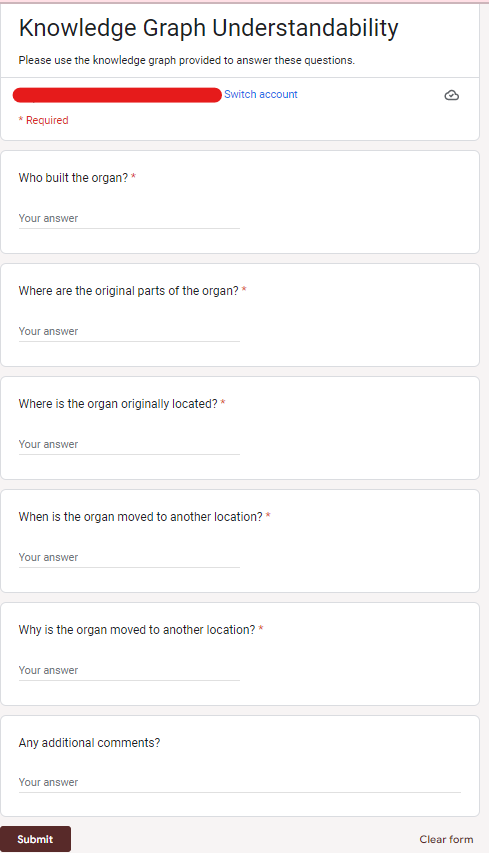
\includegraphics{Images/KGSurvey.png}
\end{center}
\vspace{-0.4cm}
\caption{Understandability Survey}
\end{figure}

\section{Knowledge Graph Understandability Example}
\lstset
{
    breaklines=true,
    breakatwhitespace=false,
    basicstyle=\linespread{1}\ttfamily,
}
\begin{lstlisting}[caption={Part01\_001MIDDE}]
@prefix fx:   <http://sparql.xyz/facade-x/ns/> .
@prefix oont: <http://w3id.org/polifonia/ontology/organs/> .
@prefix rdf:  <http://www.w3.org/1999/02/22-rdf-syntax-ns#> .
@prefix rdfs: <http://www.w3.org/2000/01/rdf-schema#> .
@prefix wd:   <https://www.wikidata.org/wiki/> .
@prefix xyz:  <http://sparql.xyz/facade-x/data/> .

"originally about a quarter lower than a1 = 440 Hz, now a1 = 466 Hz"
        oont:extraInformation  <https://organhistoricalsociety.org/OrganHistory/works/works04.htm> .

wd:Q12460259  oont:locationImage  <https://staticbrainz.org/irombook/reed_organ/reed_organ.png> .

"Hoofdwerk (II) (blockwork)"
        oont:extraInformation  <https://organhistoricalsociety.org/OrganHistory/works/works05.htm> .

"keyboard changed"
        oont:AdditionalSpecification  "Gerrit Petersz 1508" ;
        oont:Builder                  "Gerrit Petersz" ;
        oont:date                     "1508" .

"disappeared in 1886"  oont:extraInformation
                <https://organhistoricalsociety.org/OrganHistory/works/works06.htm> .

"Work division\nmain work (block work), back positive, upper work, attached pedal\n\nDisposition\n\n@Main work (II) (block work)\n\nPrestant\nOctave\nOctave@\n@\n\n16'\n8' \n4'@\n\n@Backpositive(I)\n6 voices\n\nPrestant Dd\nQuintadeen\nOctave Dd\nFlute\nMixture\nSexquialter D@\n@\n\n\n8'\n8'\n4' \n4'\n2-4 st.\n2 st.@\n\n@Bovenwerk(III)\n6 voices\n\nHolpipe\nPrincipal Dd\nOpenflute\nNasard\nGemshorn\nSifflet Dd*@\n@\n\ n\n8'\n4'\n4'\n3'\n2'\n1'@\n\n@Pedal\n1 voice\n\nTrumpet@\n@\n\n\n8'@\n\n* from a1\n\nMechanical registers\nlink HW-RP\nvalves HW, RP, BW, Ped\n\nComposition of fill voices\nMixture RP\n\nF\n1\n2/3\n\nc\n1\n2/3\ n\nc1\n1 1/3\n1 1/3\n1\n1\n\nc2\n2\n2\n1 1/3\n1 1/3\n\nSexquialter RP gis1 2 2/3 - 1 3/5 \n\nPitch\noriginally about a quarter lower than a1 = 440 Hz, now a1 = 466 Hz\nTemperature cannot be determined\n\nManual size HW FGA-c3, RP and BW FGA-g2a2\nPedal size C-d1 (C sharp, D sharp, F sharp, G sharp connected octave higher)\n\nWind supply disappeared in 1886\nWind pressure not present to be determined\n\nPlace keyboard front of main greenhouse"        oont:keyboardRange      "HW FGA-c3, RP en BW FGA-g2a2" ;
        oont:pedalRange         "C-d1 (C sharp, D sharp, F sharp, G sharp connected octave higher)" ;
        oont:pitch              "originally about a quarter lower than a1 = 440 Hz, now a1 = 466 Hz" ;
        oont:systemPlayingAids  "coupling HW-RP\nvalves HW, RP, BW, Ped" ;
        oont:temperature        "not to be determined" ;
        oont:windPressure       "not to be determined" ;
        oont:windSystem         "disappeared in 1886" .

"Koorkerk"  oont:extraInformation  <https://nl.wikipedia.org/wiki/Koorkerk> .

"disposition"  xyz:divisionName       "Hoofdwerk (II) (blockwork)" ;
        oont:AdditionalSpecification  "16'" ;
        oont:partition                "" .

"Gerrit Petersz"  oont:extraInformation
                <https://nl.wikipedia.org/wiki/Gerrit_Petersz> .

"Part01_001MIDDE"  rdf:type    wd:Q173453 , oont:Organ ;
        rdfs:subClassOf        wd:Q1327327 , wd:Q281460 , wd:Q12460259 , wd:Q752638 ;
        xyz:change             "keyboard changed" ;
        xyz:disposition        "disposition" ;
        xyz:technicals         "Work division\nmain work (block work), back positive, upper work, attached pedal\n\nDisposition\n\n@Main work (II) (block work)\n\nPrestant\nOctave\nOctave@\n@\n\n16'\n8' \n4'@\n\n@Backpositive(I)\n6 voices\n\nPrestant Dd\nQuintadeen\nOctave Dd\nFlute\nMixture\nSexquialter D@\n@\n\n\n8'\n8'\n4' \n4'\n2-4 st.\n2 st.@\n\n@Bovenwerk(III)\n6 voices\n\nHolpipe\nPrincipal Dd\nOpenflute\nNasard\nGemshorn\nSifflet Dd*@\n@\n\ n\n8'\n4'\n4'\n3'\n2'\n1'@\n\n@Pedal\n1 voice\n\nTrumpet@\n@\n\n\n8'@\n\n* from a1\n\nMechanical registers\nlink HW-RP\nvalves HW, RP, BW, Ped\n\nComposition of fill voices\nMixture RP\n\nF\n1\n2/3\n\nc\n1\n2/3\ n\nc1\n1 1/3\n1 1/3\n1\n1\n\nc2\n2\n2\n1 1/3\n1 1/3\n\nSexquialter RP gis1 2 2/3 - 1 3/5 \n\nPitch\noriginally about a quarter lower than a1 = 440 Hz, now a1 = 466 Hz\nTemperature cannot be determined\n\nManual size HW FGA-c3, RP and BW FGA-g2a2\nPedal size C-d1 (C sharp, D sharp, F sharp, G sharp connected octave higher)\n\nWind supply disappeared in 1886\nWind pressure not present to be determined\n\nPlace keyboard front main box" ;
        oont:builder           "Peter Gerritsz" ;
        oont:consolelocation   "Utrecht, Nicolaikerk" ;
        oont:creator           "Five-part construction with \"drooping shoulders\". The forms of the oldest part, the main greenhouse, are largely derived from stone architecture. Note the difference between the rather austere decoration of the frames above the towers and the rather wild, flamboyant carving on the other frames. It can clearly be seen that the pointed central tower is a later addition, especially in the carving. This consists of wave-shaped scrolls with leaf figures, an ornamentation that is typical for the mid-16th century.\nThe back positive has a raised central tower and pointed side towers with mirror fields on the inside and simple outer fields on the outside. This structure probably goes back to the backwork of the organ in the Pieterskerk in Utrecht, which was rebuilt in 1508. The carving has the same character as that of the central tower of the main work. The pediments with heads on the rugwerkkast from 1547 were in the latest fashion. Such a decoration had been installed a few years earlier in the new town hall in Utrecht. Comparable are the diamond-shaped panels with heads on the balustrade." ;
        oont:dateOfBirth       "1479" ;
        oont:extraInformation  wd:Q1444 ;
        oont:history           "Builders\n1. Peter Gerritsz\n2. Cornelis Gerritsz\n\nYears of Completion\n1. 1479\n2. 1547\n\nOriginal location Utrecht, Nicolaikerk\n\nDisposition in 1479 (probably)\n\n@Hoofdwerk\n\nBlokwerk*@\n@\n\n8'@\n\n@Bovenwerk\n\nPrincipal d \n(Cimbel?)\nPosition@\n@\n\n4'\n\n@\n@Pedal\n\nBourdonnen@\n@\n\n8'+4' tr@\n\n* 7 -18 pcs.\n\n#manual size HW H1CD-f2, BW Hcd-f2\npedal size F-e#\n\nGerrit Petersz 1508\n.keyboard changed\n\nCornelis Gerritsz 1547\n.build back positive with Prestant 8', Quintadeen 8', Octave 4', Flute 2', Mixture 3-5 st., Toesijn 8' and Schalmei 8'\n.disposition change:\nBW + Holpipe 8', + Openflute 4', + Nasard 2 2/3' , + Gemshorn 2', + Sifflet 1', + Trumpet 8'\nPed 'bourdonnen'octave removed\n.tuning changed\n.flat midfield replaced by rook, front pipes shifted\n\nDirck Petersz and Jacob Jansz van Lin 1603\ n.renovation\n.Ped + Trumpet 8'\n\nGaltus van Hagerbeer 1624\n.extensive repair work\n\nEmanuel Frederick van Montfoort 1686\n.RP + Sesquialter\n\nJohan Nicolas Heerman\n.blockwork changed\n .clutch Ped blockwork applied cht\n.old bellows replaced by four bellows from Mariakerk, Utrecht\n\nChristian Müller 1733\n.new keyboard\n.closer for the original main work installed\n\nbefore 1759\n.disposition change:\nRP - Flute\ nBW - Tertiaan 1 3/5'\n\nMaarschalkerweerd & Zn 1886\n.organ transferred to Rijksmuseum in Amsterdam\n.bellows disappeared\n\n1956\n.case with front pipes transferred to Koorkerk in Middelburg\n.other parts stored in state bunker" ;
        oont:monument          "Koorkerk" ;
        oont:monumentNumber    "28671" ;
        oont:moreInformation   "Jan van Biezen, The Dutch organ in the Renaissance and the Baroque, in particular the school of Jan van Covelens. Utrecht 1995, 708-730.\nHans Brink, Rob van der Hilst, Paul Peeters, 'Reconstruction or copying'. Criteria with regard to the transfer, 'restoration' and placement of the former organ of the Nicolaïkerk in Utrecht. Het Orgel, 78 (1982), 136-139.\nPaul Peeters, 'The Ehemalige Orgel der Nikolaikirche in Utrecht. Restore or copy?'. Acta Organologica, 22 (1991), 391-408." ;
        oont:name              "Middelburg, Koorkerk" ;
        oont:organNumber       "971" ;
        oont:particularities   "This organ retained many of its 15th and 16th century components. What remains of Peter Gerritsz is the main greenhouse, the blockwork drawer and the well boards of the main and upper work. The inner pipes and (tin) front pipes of the blockwork are also made by him. By Cornelis Gerritsz, the spring drawers of the upper work and the sliding drawers of the back positive, the well board of the back work and the register mechanism of the back positive and upper work are still present. Most of the pipework that is still present today was made by him. Below that are also the front pipes of back positive and upper. The pedal drawer is probably the Trumpet 8' by Dirck Petersz de Swart and Jacob Jansz van Lin. The lead front pipes were probably made by Galtus van Hagerbeer in 1624. The keyboard is by Christian Müller." ;
        oont:state             "Middelburg" .

wd:Q1444  wd:Property:P1343  wd:Q106727050 , wd:Q302556 ;
        wd:Property:P1535  wd:Q765778 ;
        wd:Property:P1709  <https://dbpedia.org/ontology/Organ> ;
        wd:Property:P1889  wd:Q281460 ;
        wd:Property:P2579  wd:Q11163731 ;
        wd:Property:P279   wd:Q19603939 , wd:Q52954 ;
        wd:Property:P3095  wd:Q1495811 ;
        wd:Property:P366   wd:Q60733114 , wd:Q9730 ;
        wd:Property:P527   wd:Q2927648 , wd:Q1446290 , wd:Q901207 , wd:Q25112583 , wd:Q1510738 , wd:Q392573 , wd:Q1758965 .

"not to be determined"
        oont:extraInformation  <https://organhistoricalsociety.org/OrganHistory/works/works06.htm> .

"Middelburg"  oont:extraInformation  <https://nl.wikipedia.org/wiki/Middelburg> .

\end{lstlisting} 
